\section{\ours}
\begin{figure*}[t]
\centering
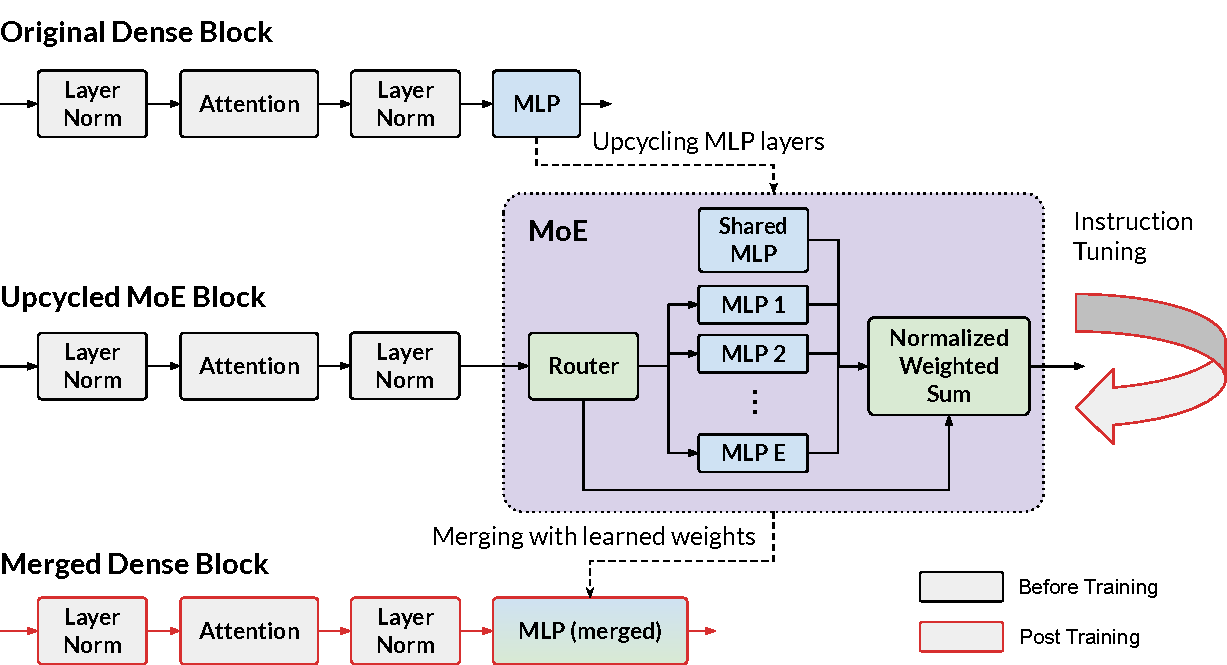
\includegraphics[width=0.8\linewidth]{assets/overview.pdf}
\caption{Overview of \ours.
}
\label{fig:overview}
\end{figure*}

We describe the details of \ours in this section. There are two steps in our framework: \textit{upcycling} (Section~\ref{sec:upcycling}) and \textit{merging} (Section~\ref{sec:merging}). During upcycling, we construct an \moefull (\moe) model from the pre-trained dense model, namely \textbf{\oursmoe}, which is then fine-tuned on coding instruction data. For merging, we propose a learnable model merging method to convert the instruction-tuned \oursmoe back to a normal dense model by merging each \moe layer into an FFN layer through weight averaging while directly copying other remaining layers. Consequently, we can obtain \textbf{\oursmerge} that has the same model architecture and size as the original pre-trained dense model, which eliminates all the additional inference overhead brought by the original \sparseupcycle, while preserving or even improving the performance of \oursmoe. Our framework is illustrated in Figure \ref{fig:overview}.

\subsection{Upcycling}\label{sec:upcycling}
Inspired by \sparseupcycle~\cite{komatsuzaki2023sparse}, we convert the pre-trained dense \llm to a new \moe by initializing each expert of each \moe layer as a copy of the original FFN layer in the dense model, while directly copying the remaining layers from the dense model to the new \moe model. However, the performance gain brought by \sparseupcycle is negligible with a very limited extra training budget~\cite{komatsuzaki2023sparse} -- which is exactly the situation we are facing during instruction tuning. Intuitively, it is because each expert in the upcycled \moe model is trained on fewer instruction data than the original dense model does because traditional routers used in \sparseupcycle will assign different tokens to different experts and thus reduce the amount of data each expert is trained on~\cite{gou2024mixture}. Consequently, inspired by \deepseekmoe~\cite{dai2024deepseekmoe} and \mocle~\cite{gou2024mixture}, \ours introduces the shared expert setting into \sparseupcycle to tackle this challenge. We further propose a novel routing weight normalization strategy for \ours to avoid the potential performance degradation caused by the scale mismatch problem~\cite{wu2022residual}.

\subsubsection{Shared Expert for Upcycling}
During upcycling, we isolate one shared expert among all the other normal experts in each \moe layer, where the shared expert will be deterministically assigned to handle all the tokens while other normal experts are assigned by the router. By doing so, the upcycled \moe model can achieve a clear performance boost in instruction tuning, where the shared expert can learn general knowledge across the whole instruction dataset while other normal experts learn specific knowledge among different instructions assigned by the router. Formally, the output hidden state $\mbox{\textbf{h}}_t^l$ of the $l$-th \moe layer when processing the $t$-th token can be expressed as:
\begin{equation}\label{formula:upcycling}
\begin{split}
\mbox{\textbf{h}}_t^l &= \sum_{i=1}^{N}(g_{i,t}\mbox{FFN}_i(\mbox{\textbf{u}}_t^l)) + \mbox{\textbf{u}}_t^l \\
g_{i,t} &= 
\begin{cases}
 1-{s_{t}}_{\max} & i=1 \\
 \mbox{Softmax}_i(s_{i,t})\cdot {s_{t}}_{\max} & s_{i,t}\in  {S_t}_K \\
    0 & {\text{otherwise}}
\end{cases} \\
{S_t}_K &= \mbox{Topk}(\{s_{i,t} \mid 1\leq i\leq N\}, K-1) \\
{s_{t}}_{\max} &= \max (\{s_{i,t} \mid 1\leq i\leq N\}) \\
s_{i,t} &= \begin{cases}
    -\infty & i = 1 \\
 \mbox{Softmax}_i({\mbox{\textbf{u}}_t^l}^T\mbox{\textbf{e}}_i^l)& i\geq 2
\end{cases} \\
\end{split}
\end{equation}
where $\textbf{h}_t^l$ refers to the output hidden state of the $l$-th \moe layer when processing the $t$-th token, $N$ refers to the total number of experts, $g_{i,t}$ refers to the gate value for the $i$-th expert, $\mbox{FFN}_i(\cdot)$ refers to the $i$-th expert, $\textbf{u}_t^l$ refers to the output hidden state of the $l$-th attention layer when processing the $t$-th token and also the input of the $l$-th \moe layer, $s_{i, t}$ refers to the affinity score between the $i$-th expert and the $t$-th token, $s_{t_{\max}}$ refers to the maximum affinity score among all the experts besides the shared expert, $\mbox{Topk}(S,K)$ refers to a function computing $K$ largest scores over $S$, $S_{tK}$ refers to a set of $K-1$ largest affinity scores among all the experts besides the shared expert, and $\textbf{e}_i^l$ refers to the centroid of the $i$-th expert in the $l$-th \moe layer.

$\mbox{FFN}_1$ is chosen as the shared expert in each \moe layer and each token will be assigned to top $K$ experts including one shared expert and $K-1$ other normal experts. Compared with the original \sparseupcycle, there are two major differences:
\begin{itemize}[leftmargin=1em]
    \setlength{\parskip}{2pt}
    \setlength\itemsep{0pt}
    \item \textbf{Weighted Shared Expert}. Following \mocle~\cite{gou2024mixture}, with the token-to-expert affinity score $s_{i,t}$, we get the maximum affinity score ${s_{t}}_{\max}$ and use its complement $1-{s_{t}}_{\max}$ as the routing weight of the shared expert.
    \item \textbf{Routing Weight Normalization}. Although the shared expert setting is also used in recent works~\cite{dai2024deepseekmoe, gou2024mixture}, we cannot directly follow their routing strategy because they cannot handle a scale mismatch problem that is unique for \sparseupcycle. The scale mismatch problem is that differences between the scale of the output of the upcycled \moe layer and the original FFN layer can cause performance degradation~\cite{wu2022residual}. To handle this problem, we need to make sure the sum of $g_{i,t}$ equals 1, so that the output of the \moe layer matches that of the FFN layer in scale. To do so, we normalize the affinity scores of top $K-1$ normal experts with Softmax and scale their sum to ${s_{t}}_{\max}$ to make sure that the sum of the $g_{i,t}$ of top $K$ experts, including one shared expert and $K-1$ normal experts, equals 1.
\end{itemize}




\subsection{Merging}\label{sec:merging}
We propose a learnable model merging method to convert the large MoE model, namely \oursmoe, back to a dense model \oursmerge. By doing so, we expect \oursmerge to keep the boosted performance gained during upcycling while keeping its model size the same as the original dense model to avoid any additional inference overhead. Inspired by \modelsoup~\cite{wortsman2022model}, we choose to merge \oursmoe by learning the mixing coefficients that can be used to average the parameters of all experts in each \moe layer to obtain a normal FFN layer, while directly copying other remaining layers. 

Formally speaking, given the weights of $N$ experts at the $l$-th layer $W_1^l, W_2^l, \cdots, W_N^l$, the process of merging each \moe layer to an FFN layer can be stated as below:
\begin{equation}\label{formula:merging1}
\begin{split}
\overline{W^l} = \sum_{i=1}^{N}\alpha_{i}^lW_{i}^l
\end{split}
\end{equation}
where $\overline{W^l}$ denotes the merged parameter of all $N$ experts and $\alpha_i^l$ denotes the learnable mixing coefficient of expert $W_i^l$. We consider a neural network $f(x; \theta)$ with input $x$ and parameters $\theta$. For loss $\mathcal{L}$ and instruction dataset $\{(x_i,y_i)\}_{i=1}^m$, such mixing coefficients $\alpha$ of all the $L$ layers can be learned via:
\begin{equation}\label{formula:merging2}
\begin{split}
\arg\min_{\alpha}\sum_{j=1}^{m}\mathcal{L}(f(x_j; \theta_{o}, (\sum_{i=1}^{N}\alpha_{i}^lW_{i}^l)_{1:L}), y_i)
\end{split}
\end{equation}
where $\theta_{o}$ refers to all the remaining layers of \oursmoe other than \moe layers and $\alpha$ is parameterized as the output of a softmax, so that each $\alpha_i^l$ is positive and $\sum_{i=1}^N\alpha_i^l = 1$.

While the learning process defined in Eq. (\ref{formula:merging2}) is the most intuitive way of learning $\alpha$, our experiment in Section \ref{sec:ablation_merging} shows that, due to the shared expert setting, it tends to simply increase the mixing coefficient of the shared expert at each layer as much as possible to decrease the loss. It is not helpful because, although the shared expert has learned general knowledge across the whole instruction dataset and needs a relatively large mixing coefficient, we still need to keep the scale of the mixing coefficient of other normal experts at a certain level also to keep some specific knowledge learned by other normal experts in the merged parameter $\overline{W^l}$.

To solve this issue, we introduce a \textit{shared expert rate} $\lambda$ to fix the mixing coefficient of the shared expert and learn the mixing coefficients of the remaining normal experts which sums to $1-\lambda$ in each layer. By doing so, we can easily control the scale of the mixing coefficient of the shared expert, while still being able to learn the optimal layer-wise mixing coefficients of other normal experts. Let's say $W_1^l$ is the shared expert of the $l$-th layer, then Eq. (\ref{formula:merging1}) and Eq. (\ref{formula:merging2}) can be reformulated as below:
\begin{gather}
\overline{W^l} = \lambda W_{1}^l + \sum_{i=2}^{N}\alpha_{i}^lW_{i}^l\label{formula:merging1new}\\
\arg\min_{\alpha}\sum_{j=1}^{m}\mathcal{L}(f(x_j; \theta_o, \overline{W^l}_{1:L}), y_i)\label{formula:merging2new}
\end{gather}

In practice, we uniformly initialize the mixing coefficients $\alpha$ of all the normal experts as $\frac{1-\lambda}{N-1}$, which is then trained on the same instruction dataset as upcycling.
